\documentclass[12pt]{article}

\usepackage[utf8]{inputenc}
\usepackage[T1]{fontenc}
\usepackage{lmodern}
\usepackage[fleqn]{mathtools}
\usepackage{amssymb}
\usepackage[margin=1.0in]{geometry}
\usepackage{xparse}
\usepackage{parskip}
\usepackage[compact]{titlesec}
\usepackage{tikz}
\usetikzlibrary{matrix}

\DeclarePairedDelimiter\abs{\lvert}{\rvert}
\DeclarePairedDelimiter\paren{(}{)}

\setlength{\parindent}{0pt}
\setlength{\mathindent}{0pt}

\titleformat*{\subsection}{\bfseries}

\let\oldimplies\implies%
\renewcommand*{\implies}{\Rightarrow}
\newcommand*{\R}{\mathbb{R}}
\newcommand*{\asin}{\sin^{-1}}
\newcommand*{\acos}{\cos^{-1}}
\newcommand*{\atan}{\tan^{-1}}
\DeclareDocumentCommand{\dd}{O{}om}{\IfNoValueTF{#2}{\tfrac{\mathrm{d}#1}%
  {\mathrm{d}#3}}{\tfrac{\mathrm{d}^{#1}#2}{\mathrm{d}#3^{#1}}}}
\newcommand*{\D}[1]{\mathop{}\!\mathrm{d}#1}
\newcommand*{\isum}[1]{\sum\limits_{#1}^\infty}
\newcommand{\pvec}[1]{\vec{#1}\mkern2mu\vphantom{#1}}
\makeatletter
\newcommand{\mquote}[1]{{\mathpalette\mqu@te{#1}}}
\newcommand{\mqu@te}[2]{%
  \sbox0{\(\m@th#1\text{``}\)}%
  \sbox1{\(\m@th#1\text{''}\)}%
  \sbox2{\(\m@th#1#2\)}%
  \ifdim\ht2>\ht0
    \raisebox{\dimexpr\ht2-\height}{\box0}%
    #2%
    \raisebox{\dimexpr\ht2-\height}{\box1}%
  \else
    \box0 #2\box1
  \fi
}
\makeatother

\newcommand*{\fixmath}{%
  \makebox{}\vspace{\glueexpr-\baselineskip-\abovedisplayskip}}
\newenvironment{fixaskip}{\setlength{\abovedisplayskip}{0pt}\fixmath%
  \ignorespaces}{\ignorespacesafterend}
\newenvironment{fixbskip}{\setlength{\belowdisplayskip}{0pt}\ignorespaces}%
  {\ignorespacesafterend}
\newenvironment{fixskip}{\setlength{\abovedisplayskip}{0pt}%
  \setlength{\belowdisplayskip}{0pt}\fixmath\ignorespaces}%
  {\ignorespacesafterend}

\begin{document}
\section*{Double Angle Formulas}
\begin{fixskip}
  \begin{align*}
    \sin(2x) &= 2\sin(x)\cos(x)\\
    \cos(2x) &= \cos^2(x) - \sin^2(x)\\
      &= 2\cos^2(x) - 1\\
      &= 1-2\sin^2(x)\\
    \tan(2x) &= \frac{2\tan(x)}{1 - \tan^2(x)}\\
    \sin^2(x) &= \frac{1}{2}(1-\cos(2x))\\
    \cos^2(x) &= \frac{1}{2}(1+\cos(2x))
  \end{align*}
\end{fixskip}
\section*{Limits}
\begin{fixaskip}
  \[
    \lim_{x \to n} f(x) = L
  \]
\end{fixaskip}
Means for any number \(\epsilon > 0\) there exists a number \(\delta > 0\) such
that if \(0 < \abs*{x-n} < \delta\) then \(\abs*{f(x)-L} < \epsilon\).
\[
  \lim_{x \to a}f(g(x)) = f\paren*{\lim_{x \to a}g(x)} \text{ if } f(g(x))
  \text{ is continuous at } x
\]
Standard difference quotient:
\[
  f'(x) = \lim_{h \to 0}\frac{f(x+h) - f(x)}{h}
\]
Symmetric difference quotient:
\begin{fixbskip}
  \[
    f'(x) = \lim_{h \to 0}\frac{f(x+h) - f(x-h)}{2h}
  \]
\end{fixbskip}
\section*{Continuity and Differentiability}
\(f(x)\) is continuous at \(x\) if:
\[
  f(x) = \lim_{k \to x^+}f(k) = \lim_{k \to x^-}f(k)
\]
\(f(x)\) is differentiable at \(x\) if:
\begin{fixbskip}
  \[
    f'_+(x) = f'_-(x)
  \]
\end{fixbskip}
\section*{Differentiation Rules}
\begin{fixskip}
  \begin{align*}
    \dd{x}c f(x) &= c f'(x)\\
    \dd{x}f(g(x)) &= f'(g(x))g'(x)\\
    \dd{x}(f(x) \pm g(x)) &= f'(x) \pm g'(x)\\
    \dd{x}{f(x)}^n &= n{f(x)}^{n-1} \cdot f'(x)\\
    \dd{x}\sqrt{f(x)} &= \frac{f'(x)}{2\sqrt{f(x)}}\\
    \dd{x}(f(x)g(x)) &= f'(x)g(x) + f(x)g'(x)\\
    \dd{x}\paren*{\frac{f(x)}{g(x)}} &= \frac{f'(x)g(x) - f(x)g'(x)}
      {{g(x)}^2}\\
    \dd{x}\abs*{f(x)} &= \frac{\abs*{f(x)}}{f(x)} \cdot f'(x)\\
    \dd{x}b^{f(x)} &= b^{f(x)} \ln b \cdot f'(x)\\
    \dd{x}\log_b(f(x)) &= \frac{f'(x)}{f(x) \ln b}
  \end{align*}
\end{fixskip}
\section*{Trigonometric Differentiation Rules}
\begin{fixskip}
  \begin{align*}
    \dd{x}\sin(f(x)) &= \cos(f(x)) \cdot f'(x)\\
    \dd{x}\cos(f(x)) &= -\sin(f(x)) \cdot f'(x)\\
    \dd{x}\tan(f(x)) &= \sec^2(f(x)) \cdot f'(x)\\
    \dd{x}\sec(f(x)) &= \sec(f(x))\tan(f(x)) \cdot f'(x)\\
    \dd{x}\csc(f(x)) &= -\csc(f(x))\cot(f(x)) \cdot f'(x)\\
    \dd{x}\cot(f(x)) &= -\csc^2(f(x)) \cdot f'(x)
  \end{align*}
\end{fixskip}
\section*{Inverse Trigonometric Differentiation Rules}
\begin{fixskip}
  \begin{align*}
    \dd{x}\asin(f(x)) &= \frac{f'(x)}{\sqrt{1 - {f(x)}^2}}\\
    \dd{x}\acos(f(x)) &= -\frac{f'(x)}{\sqrt{1 - {f(x)}^2}}\\
    \dd{x}\atan(f(x)) &= \frac{f'(x)}{1 + {f(x)}^2}
  \end{align*}
\end{fixskip}
\section*{Mean Value Theorem}
If \(f(x)\) is continuous on \([a,b]\), then there exists one value \(c\) on
\([a,b]\) such that:
\begin{fixbskip}
  \[
    f'(c) = \frac{f(b) - f(a)}{b - a}
  \]
\end{fixbskip}
\section*{Reimann Sums}
\begin{fixaskip}
  \[
    \sum_{k=1}^n f(x_k) \Delta x\\
  \]
\end{fixaskip}
Assuming regular partition:
\begin{fixbskip}
  \begin{align*}
    \text{LRAM} &= \sum_{k=1}^n f\paren*{a + \frac{(k-1)(b - a)}{n}}
      \frac{b-a}{n}\\
    \text{MRAM} &= \sum_{k=1}^n f\paren*{a + \frac{(k-\frac{1}{2})(b - a)}{n}}
      \frac{b-a}{n}\\
    \text{RRAM} &= \sum_{k=1}^n f\paren*{a + \frac{k(b - a)}{n}}
      \frac{b-a}{n}
  \end{align*}
\end{fixbskip}
\section*{Definite Integration}
\begin{fixaskip}
  \begin{align*}
    \int_a^b f(x) \D{x} &= \lim_{n \to \infty} \sum_{k=1}^n f(x_k)\Delta x\\
    \int_a^a f(x) \D{x} &= 0\\
    \int_a^b f(x) \D{x} &= -\int_b^a f(x) \D{x}\\
    \int_a^b c f(x) \D{x} &= c \int_a^b f(x) \D{x}\\
    \int_a^b (f(x) \pm g(x)) \D{x} &= \int_a^b f(x) \D{x} \pm \int_a^b g(x)
      \D{x}\\
    \int_a^p f(x) \D{x} + \int_p^b f(x) \D{x} &= \int_a^b f(x) \D{x}\\
    \int_a^b f(x) \D{x} &> \int_a^b g(x) \D{x} \text{ if }f(x) > g(x)
      \text{ on } [a,b]
  \end{align*}
\end{fixaskip}
The mean value of \(f(x)\) over \([a,b]\) is:
\begin{fixbskip}
  \[
    \frac{1}{b - a} \int_a^b f(x) \D{x}
  \]
\end{fixbskip}
\section*{Mean Value of a Function Theorem}
If \(f(x)\) is continuous on \([a,b]\), then there exists one value \(c\) on
\([a,b]\) such that:
\begin{fixbskip}
  \[
    f(c) = \frac{1}{b - a} \int_a^b f(x) \D{x}
  \]
\end{fixbskip}
\section*{Linear Approximation}
The linearization of \(f(x)\) at \(a\):
\begin{fixbskip}
  \[
    L(x) = f(a) + f'(a)(x-a)
  \]
\end{fixbskip}
\section*{Fundamental Theorem of Calculus}
\subsection*{Part 1}
\begin{fixskip}
  \[
    \dd{x} \int_{a(x)}^{b(x)} f(t) \D{t} = f(b(x)) b'(x) - f(a(x)) a'(x)
  \]
\end{fixskip}
\subsection*{Part 2}
\begin{fixskip}
  \begin{align*}
    F'(x) &= f(x)\\
    \int_a^b f(x) &= F(x) \bigg|_a^b = F(b) - F(a)
  \end{align*}
\end{fixskip}
\section*{Solving Differential Equations Using A Definite Integral}
\begin{fixaskip}
  \begin{align*}
    \dd[y]{x} &= f(x)\\
    y &= \int_a^x f(t) \D{t} + C
  \end{align*}
\end{fixaskip}
The easiest solution occurs when \(a = \) the given \(x\) value and \(C = \)
the given \(y\) value.
\section*{Solving Differential Equations Using Antidifferentiation}
\begin{fixaskip}
  \begin{align*}
    \dd[y]{x} &= f(x)\\
    y &= \int f(x) + C \text{ (general form)}
  \end{align*}
\end{fixaskip}
Specify largest domain of \(x\) that includes specified \(x\) and does not
include any discontinuities.
\section*{Euler's Method}
Start at \((x_0,y_0)\)
\begin{fixbskip}
  \begin{align*}
    \Delta y &= \Delta x \cdot \dd[y]{x} \bigg|_{(x_{n-1},y_{n-1})}\\
    (x_n,y_n) &= (x_{n-1} + \Delta x, y_{n-1} + \Delta y)
  \end{align*}
\end{fixbskip}
\section*{Antidifferentiation Rules}
\begin{fixskip}
  \begin{align*}
    \int cf(x) \D{x} &= c \int f(x) \D{x}\\
    \int f(x) \pm g(x) \D{x} &= \int f(x) \D{x} \pm \int g(x) \D{x}\\
    \int x^n \D{x} &= \frac{x^{n+1}}{n+1} + C\\
    \int \frac{1}{x} \D{x} &= \ln\abs*{x} + C\\
    \int b^x \D{x} &= \frac{b^x}{\ln b} + C\\
    \int \ln x \D{x} &= x\ln x - x + C
  \end{align*}
\end{fixskip}
\section*{Trigonometric Antidifferentiation Rules}
\begin{fixskip}
  \begin{align*}
    \int \sin(x) \D{x} &= -\cos(x) + C\\
    \int \cos(x) \D{x} &= \sin(x) + C\\
    \int \tan(x) \D{x} &= -\ln\abs*{\cos(x)} + C\\
    \int \sec(x) \D{x} &= \ln\abs*{\sec(x)+\tan(x)} + C\\
    \int \sin^2(x) \D{x} &= \frac{1}{2} (x - \sin(x)\cos(x)) + C\\
    \int \cos^2(x) \D{x} &= \frac{1}{2} (x + \sin(x)\cos(x)) + C\\
    \int \tan^2(x) \D{x} &= \tan(x) - x + C\\
    \int \sec^2(x) \D{x} &= \tan(x) + C\\
    \int \sec(x) \tan(x) \D{x} &= \sec(x) + C\\
    \int \frac{1}{1+x^2} \D{x} &= \atan(x) + C\\
    \int \frac{1}{\sqrt{1-x^2}} \D{x} &= \asin(x) + C
  \end{align*}
\end{fixskip}
\section*{Inverse Trigonometric Antidifferentiation Rules}
\begin{fixskip}
  \begin{align*}
    \int \asin(x) &= x\asin(x) + \sqrt{1-x^2}\\
    \int \atan(x) &= x\atan(x) - \frac{1}{2} \ln(1 + x^2) + C
  \end{align*}
\end{fixskip}
\section*{U-Substitution}
To differentiate \(\int f(g(x)) \D{x}\) where \(f(x)\) and \(g(x)\) are both
antidifferentiable, set \(u = g(x)\). Then solve for \(du\) and replace \(dx\)
so that the equation \(A\int f(u) \D{u}\) results (where \(A\) is the necessary
``fudge factor''). Antidifferentiate and replace \(u\) with \(g(x)\).
\section*{Integration by Parts}
\begin{fixaskip}
  \[
    \int u \D{v} = uv - \int v \D{u} + C
  \]
\end{fixaskip}

or

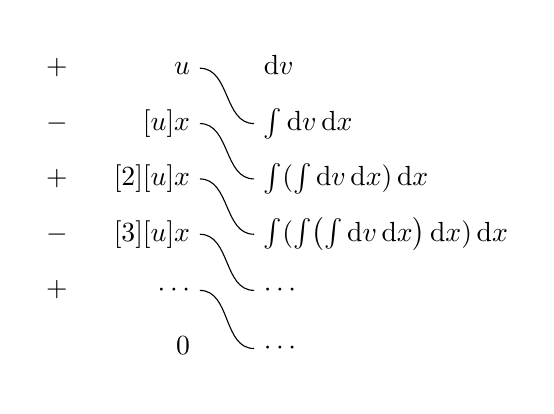
\begin{tikzpicture}
  \matrix[matrix of nodes,
    nodes={minimum height=2em},
    column sep=1em,
    column 2/.style={anchor=base east},
    column 3/.style={anchor=base west}]{
    \(+\) & |(d0)| \(u\) &[1em] \(\D{v}\)\\
    \(-\) & |(d1)| \(\dd[u]{x}\) & |(i1)| \(\int \D{v} \D{x}\)\\
    \(+\) & |(d2)| \(\dd[2][u]{x}\) &
      |(i2)| \(\int(\int\D{v}\D{x})\D{x}\)\\
    \(-\) & |(d3)| \(\dd[3][u]{x}\) &
      |(i3)| \(\int(\int\paren*{\int\D{v}\D{x}}\D{x})\D{x}\)\\
    \(+\) & |(d4)| \(\cdots\) & |(i4)| \(\cdots\)\\
          & 0 & |(i5)| \(\cdots\)\\
  };
  \foreach \d/\i in {d0/i1,d1/i2,d2/i3,d3/i4,d4/i5}{
    \draw (\d) to[out=0,in=180] (\i);
  }
\end{tikzpicture}
\begin{fixbskip}
  \[
    \int u \D{v} = \paren*{u \cdot \int \D{v} \D{x}}
      - \paren*{\dd[u]{x} \cdot \int \paren*{ \int \D{v} \D{x}} \D{x}}
      + \paren*{\dd[2][u]{x} \cdot \int \paren*{\int \paren*{\int \D{v} \D{x}}
        \D{x}} \D{x}} - \cdots
  \]
\end{fixbskip}
\section*{Partial Fraction Decomposition}
Convert fractions of form \(\frac{\text{linear or constant}}{\text{factorable
quadratic}}\) into its partial fraction.
\begin{align*}
  \frac{h(x)}{f(x)g(x)} &= \frac{A}{f(x)} + \frac{B}{g(x)} = \frac{Ag(x)}
  {f(x)g(x)} + \frac{Bf(x)}{f(x)g(x)} = \frac{Ag(x) + Bf(x)}{f(x)g(x)}\\
  h(x) &= Ag(x) + Bf(x)
\end{align*}
Choose a value of \(x\) such that \(f(x) = 0\) and then \(g(x) = 0\) to solve
for \(A\) and \(B\) respectively.
\section*{Exponential Growth\slash Decay}
\begin{fixskip}
  \begin{align*}
    \dd[Q]{t} &= kQ\\
    Q &= Q_0 e^{kt} = Q_0 b^{\frac{t}{p}}\\
    k &= -\frac{\ln(b)}{p}
  \end{align*}
\end{fixskip}
\subsection*{Half-life}
\begin{fixskip}
  \[
    k = -\frac{\ln(2)}{p}
  \]
\end{fixskip}
\section*{Logistic Differential Equation}
\begin{fixaskip}
  \[
    \dd[P]{t} = kP(m - P) = kPm\paren*{1-\frac{P}{m}}
  \]
\end{fixaskip}
where \(P\) is the population and \(M\) is the carrying capacity
\[
  P(t) = \frac{m}{1 + Ae^{-mkt}}
\]
The maximum carrying capacity is reached when \(P(t) = m - 0.5\), if \(P(0) <
m\), or right after \(P(t) = m + 0.5\), if \(P(0) > m\).
\section*{Calculating Area of Regions Bounded by Two Functions}
\begin{fixaskip}
  \[
    A = \int_a^b f(x) - g(x) \D{x}
  \]
\end{fixaskip}
where \(f(x)\) is the upper function and \(g(x)\) is the lower function.

If the functions cross, multiple integrals must be taken with the appropriate
upper and lower functions.
\section*{Typical Cross-Sectional Areas}
{\renewcommand{\arraystretch}{1.5}\begin{tabular}{l@{ }l}
  Square: & \(A = b^2 = \frac{1}{2}d^2\)\\
  Rectangle: & \(A = bh\)\\
  Equalateral triangle: & \(A = \frac{\sqrt{3}}{4}b^2\)\\
  Right isoceles triangle: & \(A = \frac{1}{2}l^2 = \frac{1}{4}h^2\)\\
  Hexagon: & \(A = \frac{3\sqrt{3}}{2} s^2\)\\
  Circle: & \(A = \pi r^2 = \frac{1}{4}\pi d^2\)\\
  Semicircle: & \(A = \frac{1}{2}\pi r^2 = \frac{1}{8}\pi d^2\)\\
  Parabolic region: & \(A = \frac{2}{3}bh\)
\end{tabular}}
\section*{Calculating Volume Using the Disk\slash Washer Method for Solids of
Rotation}
\begin{fixaskip}
  \[
    V = \pi\int_a^b r_{\text{outer}}^2 - r_{\text{inner}}^2 \D{t}
  \]
\end{fixaskip}
where \(\D{t}\) is the differential thickness of the disk\slash washer.
\section*{Calculating Volume Using the Cylindrical Shell Method for Solids of
Rotation}
\begin{fixaskip}
  \[
    V = 2\pi \int_a^b hr \D{t}
  \]
\end{fixaskip}
where \(\D{t}\) is the differential thickness of the shell.
\section*{Calculating Arc Lengh}
\begin{fixbskip}
  \[
    l = \int_a^b \sqrt{1+{\paren*{\dd[y]{x}}}^2} \D{x}
    = \int_c^d \sqrt{1+{\paren*{\dd[x]{y}}}^2} \D{y}
  \]
\end{fixbskip}
\section*{L'H\^{o}pitals Rule}
In order to evaluate a limit where
\[
  \lim_{x \to a} \frac{f(x)}{g(x)} \implies \mquote{\frac{0}{0}} \text{ or }
  \mquote{\frac{\infty}{\infty}}
\]
evaluate
\[
  \lim_{x \to a} \frac{f'(x)}{g'(x)}
\]
In order to evaluate a limit where
\[
  \lim_{x \to a} {f(x)}^{g(x)} \implies \mquote{0^0} \text{ or }
  \mquote{1^\infty} \text{ or } \mquote{\infty^0}
\]
set \(L\) equal to the original limit and immediately take the log of both
sides
\begin{align*}
  L &= \lim_{x \to a} {f(x)}^{g(x)}\\
  \ln(L) &= \ln\paren*{\lim_{x \to a} {f(x)}^{g(x)}}\\
  \ln(L) &= \lim_{x \to a} g(x) \ln f(x)
\end{align*}
Evaluate the resulting limit and then raise \(e\) to that result
\section*{Relative Rates of Growth}
To compare rates of \(f(x)\) and \(g(x)\) evaluate
\begin{fixbskip}
  \[
    \lim_{x \to \infty} \frac{f(x)}{g(x)} = \begin{dcases*}
      \infty & then \(f(x)\) grows faster than \(g\)\\
      \left<0, \infty\right> & then \(f(x)\) and \(g(x)\) grow at the same
        rate\\
      0 & then \(f(x)\) grows slower than \(g(x)\)
    \end{dcases*}
  \]
\end{fixbskip}
\section*{Improper Integrals}
\subsection*{Type 1}
\begin{fixskip}
  \begin{align*}
    \int_a^\infty f(x) \D{x} &= \lim_{n \to \infty} \int_a^n f(x) \D{x}\\
    \int_{-\infty}^b f(x) \D{x} &= \lim_{n \to \infty} \int_{-n}^b f(x) \D{x}\\
    \int_{-\infty}^\infty f(x) \D{x} &= \lim_{n \to \infty} \int_{-n}^n f(x)
      \D{x}
  \end{align*}
\end{fixskip}
\subsection*{Type 2}
\begin{fixaskip}
  \[
    \int_a^b f(x)
  \]
\end{fixaskip}
such that there is at least one vertical-asymptotic discontinuity on \([a,b]\).
\begin{alignat*}{3}
  &\int_a^b f(x) \D{x} \text{ (where discontinuity at \(a\)) }
    &&= \lim_{n \to a^+} \int_n^b f(x) \D{x}\\
  &\int_a^b f(x) \D{x} \text{ (where discontinuity at \(b\)) }
    &&= \lim_{n \to b^-} \int_a^n f(x) \D{x}\\
  &\int_a^b f(x) \D{x} \text{ (where discontinuity \(d\) on
    \(\left<a,b\right>\)) } &&= \lim_{n \to d^-} \int_a^n f(x) \D{x} +
    \lim_{n \to d^+} \int_n^b f(x) \D{x}
\end{alignat*}
\subsection*{P-Integrals}
An integral that fits the pattern:
\[
  \int_1^\infty \frac{1}{x^p} \D{x} \text{ where \(p\) is positive}
\]
\begin{fixaskip}
  \begin{align*}
    p > 1 &\implies \text{the integral converges to \(\tfrac{1}{p-1}\).}\\
    0 < p \le 1 &\implies \text{the integral diverges.}
  \end{align*}
\end{fixaskip}
\section*{Comparison Tests}
For positive type 1 improper integrals (\(a = \infty\) and\slash or
\(b = \infty\)) where the integrand is not easily antidifferentiable:
\[
  \int_a^b f(x) \D{x}
\]
Establish bound functions which can be antidifferentiated:
\[
  l(x) \le f(x) \le u(x)
\]
\begin{fixskip}
  \begin{alignat*}{3}
    \text{Convergence if } &\int_a^b f(x) \D{x} \le \int_a^b u(x) \D{x}
      &&\text{ and } \int_a^b u(x) \D{x} \text{ converges}\\
    \text{Divergence if } &\int_a^b f(x) \D{x} \ge \int_a^b l(x) \D{x}
      &&\text{ and } \int_a^b l(x) \D{x} \text{ diverges}
  \end{alignat*}
\end{fixskip}
\section*{Sequences}
\subsection*{Explicit Definition}
\begin{fixaskip}
  \[
    x_k = f(k)
  \]
\end{fixaskip}
where \(k \in \{1,2,3,\dots\}\).
\subsection*{Recursive Definition}
\begin{fixaskip}
  \[
    x_k = m(x_{k-1})
  \]
\end{fixaskip}
where \(x_1\) is defined and \(k \in \{2,3,4,\dots\}\).
\subsection*{Arithmetic}
\begin{fixskip}
  \begin{align*}
    x_k &= d(k-1) + x_1\\
    x_k &= t_{k-1} + d
  \end{align*}
\end{fixskip}
\subsection*{Geometric}
\begin{fixskip}
  \begin{align*}
    x_k &= x_1r^{k-1}\\
    x_k &= x_{k-1} r
  \end{align*}
\end{fixskip}
\subsection*{Convergence\slash Divergence}
A sequence converges if the limit \(\displaystyle\lim_{n \to \infty} x_n\) is
a finite number else it diverges.
\section*{Infinite Series}
\begin{fixskip}
  \[
    \isum{k=0} x_k
  \]
\end{fixskip}
\subsection*{Convergence}
Consider the sequence of ``partial sums'' (\(s\)) where:
\[
  s_n = \sum_{k=0}^n x_k
\]
If \(\{s_n\}\) converges to \(S\) then the infinite series converges to \(S\).
\subsection*{Power Series}
\begin{fixskip}
  \[
    \isum{k=0} c_k{(x-a)}^k
  \]
\end{fixskip}
\subsection*{Taylor\slash Maclaurin Series}
Given an infinitely differentiable function \(f(x)\), the Taylor series
centered around \(a\) is equal to the power series with a specific \(c_k\):
\[
  f(x) = \isum{k=0} \frac{f^{(k)}(a)}{k!}{(x-a)}^k
\]

A Maclaurin series is a Taylor series centered around 0 (\(a = 0\)).

The \(n\)-order polynomial function \(P_n(x)\) that best fits \(f(x)\) is
equal to the Taylor series evaluated with upper limit \(n\):
\[
  P_n(x) = \sum_{k=0}^{n} \frac{f^{(k)}(a)}{k!}{(x-a)}^k
\]
\subsection*{Common Maclaurin Series}
\begin{fixskip}
  \begin{alignat*}{3}
    \frac{a}{1-x} &= \isum{k=0} ax^k &&\quad x \in \left<-1,1\right>\\
    e^x &= \isum{k=0} \frac{x^k}{k!} &&\quad x \in \R\\
    \sin(x) &= \isum{k=0} {(-1)}^k \frac{x^{2k+1}}{(2k+1)!} &&\quad x \in \R\\
    \cos(x) &= \isum{k=0} {(-1)}^k \frac{x^{2k}}{(2k)!} &&\quad x \in \R\\
    \atan(x) &= \isum{k=0} {(-1)}^k \frac{x^{2k+1}}{2k+1} &&\quad x \in [-1,1]\\
    \ln(x+1) &= \isum{k=1} {(-1)}^{k+1} \frac{x^k}{k} &&\quad x \in
      \left<-1,1\right]
  \end{alignat*}
\end{fixskip}
\subsection*{Calculating Error for a Taylor Polynomial}
\begin{fixaskip}
  \[
    P_\infty(x) = P_n(x) + R_n(x)
  \]
\end{fixaskip}
where \(P_\infty\) is the entire infinite Taylor series and \(R_n\) is the
remainder (note that the remainder series starts with \(k=n+1\)).

Lagrange Error:
\begin{align*}
  R_n(x) &= \frac{f^{(n+1)}(c)}{(n+1)!}{(x-a)}^{n+1}
    \quad\text{for an unknown \(c \in \left<a,x\right>\).}\\
  \abs*{R_n(x)} &= \abs*{\frac{f^{(n+1)}(c)}{(n+1)!}{(x-a)}^{n+1}}\\
  \abs*{R_n(x)} &= \frac{\abs*{f^{(n+1)}(c)}}{(n+1)!}\abs*{x-a}^{n+1}
\end{align*}


To bound the error:
\[
  \abs*{R_n(x)} \le \frac{M}{(n+1)!}\abs*{x-a}^{n+1}
\]
Where \(M\) is a positive number greater than or equal to every possible value
\(f^{(n+1)}(t)\) where \(t\) is in the interval of study.

The series then converges if:
\[
  \lim_{n \to \infty} \abs*{R_n(x)} = 0
\]
\section*{Infinite Series Tests}
\subsection*{n\textsuperscript{th}-Term Test}
If \(\lim\limits_{n \to \infty} a_n \ne 0\), the series
\(\isum{n=0}a_n\) diverges.
\subsection*{Comparison Test}
To conclude whether a series \(S\) converges or diverges establish a known
series \(T\).
\begin{fixbskip}
  \begin{align*}
    \text{Convergence if } &S \le T \text{ and } S \text { converges}\\
    \text{Divergence if } &S \ge T \text{ and } S \text { diverges}
  \end{align*}
\end{fixbskip}
\subsection*{Alternating Test}
Any alternating series that passes the n\textsuperscript{th}-term test where
the magnitude of successive terms decreases will converge.

A series which depends on alternation has conditional convergence. A series
which converges whether all terms are positive or negative has absolute
convergence.

Additionally the error is less than the next term in the sequence for an
alternating sequence.
\subsection*{P-Series Test}
If the series is in the form \(a_n = \frac{1}{n^p}\), then if \(p > 1\) the
series converges, else it diverges.
\subsection*{Telescoping Series Test}
For a series where subsequent terms cancel out previous terms such as:
\[
  \isum{k=1} \frac{1}{(k)(k+1)}
\]
Separate into partial fractions:
\[
  \isum{k=1} \frac{1}{k}-\frac{1}{k+1} = \paren*{\frac{1}{1} - \frac{1}{2}} +
  \paren*{\frac{1}{2} - \frac{1}{3}} + \paren*{\frac{1}{3} - \frac{1}{4}}
  + \cdots + \paren*{\frac{1}{n} - \frac{1}{n+1}}
  = 1 - \frac{1}{n+1}
\]
\subsection*{Ratio Test}
For a series:
\[
  \isum{k=0} t_k \text{ where } t_k \ge 0
\]
consider
\[
  \lim_{k \to \infty} \frac{t_{k+1}}{t_k} = \begin{dcases*}
    \left[0,1\right> & the series converges\\
    1 & the test is inconclusive\\
    \left<1,\infty\right> \text{ or } \infty  & the series is divergent
  \end{dcases*}
\]
To evaluate for a power series take the absolute value of the ratio:
\[
  \lim_{k \to \infty} \abs*{\frac{c_{k+1}{(x-a)}^{k+1}}{c_k{(x-a)}^k}}
  = \lim_{k \to \infty} \abs*{\frac{c_{k+1}}{c_k}}\abs*{x-a}
\]
Then to find radius of convergence:
\[
  l = \lim_{k \to \infty} \abs*{\frac{c_{k+1}}{c_k}} = \begin{dcases*}
    0 & the series converges for \(x \in \mathbb{R}\)\\
    \left<0,\infty\right> & the series converges for
      \(\abs*{x-a} < R = \tfrac{1}{l}\)\\
    \infty & the series converges only for \(x=a\)
  \end{dcases*}
\]
\subsection*{Integral Test}
Find positive, continuous, and decreasing function where \(f(n) = a_n\). If
\(\int\limits_0^\infty f(x) \D{x}\) converges the series will converge; if it
diverges the series will diverge.
\section*{Parametric Functions}
Both \(x\) and \(y\) defined in terms of third variable:
\begin{align*}
  x &= f(t)\\
  y &= g(t)
\end{align*}
\subsection*{Eliminating the Parameter}
Solve the for \(t\) in one of the equaitons and substitute or find another way
to combine the two equations to eliminate \(t\);
\subsection*{Taking Derivatives}
\begin{fixaskip}
  \begin{align*}
    \dd[y]{x} &= \frac{\dd[y]{t}}{\dd[x]{t}}\\
    \dd[2][y]{x} &= \frac{\dd{t}\paren*{\dd[y]{x}}}{\dd[x]{t}}
  \end{align*}
\end{fixaskip}
\subsection*{Calculating Arc Length}
\begin{fixskip}
  \[
    \int_{t_1}^{t_2}\sqrt{\paren*{\dd[x]{t}}^2 + \paren*{\dd[y]{t}}^2}\D{t}
  \]
\end{fixskip}
\section*{Polar Functions}
Points are identified by radius \(r\) and angle \(\theta\): \((r,\theta)\).
There exist infinitely many polar representations for the same point.

Equations are usually \(r\) in terms of \(\theta\): \(r = f(\theta)\).
\subsection*{Relationships With Cartesian Points}
\begin{fixskip}
  \begin{align*}
    r &= \sqrt{x^2+y^2}\\
    x &= r\cos(\theta)\\
    y &= r\sin(\theta)
  \end{align*}
\end{fixskip}
\subsection*{Calculating Instantaneous Slope}
\begin{fixskip}
  \[
    \dd[y]{x} = \frac{\dd[y]{\theta}}{\dd[x]{\theta}}
    = \frac{\dd{\theta}(r\sin(\theta))}{\dd{\theta}(r\cos(\theta))}
    = \frac{\dd[r]{\theta}\sin(\theta) + r\cos(\theta)}%
      {\dd[r]{\theta}\cos(\theta) - r\sin(\theta)}
  \]
\end{fixskip}
\subsection*{Calculating Area Bounded by Curve}
\begin{fixskip}
  \[
    \frac{1}{2} \int_\alpha^\beta {(r(\theta))}^2 \D{\theta}
  \]
\end{fixskip}
\section*{Vector Functions}
\begin{fixaskip}
  \begin{gather*}
    \vec{s}(t) = \left<f(t),g(t)\right>\\
    \pvec{s}'(t) = \vec{v}(t) = \left<f'(t),g'(t)\right>\\
    \pvec{s}''(t) = \pvec{v}'(t) = \vec{a}(t) = \left<f''(t),g''(t)\right>
  \end{gather*}
\end{fixaskip}
\[
  \text{speed} = \abs{\vec{v}} = \sqrt{{(f'(t))}^2 + {(g'(t))}^2}
\]
\end{document}
